\newpage
\chapter{Materials and Methods}
\label{sec:Approach}

\section{General Problem Formulation}
\label{sec:Approach_GPF}
The general idea behind \ac{TAD} is that a high-dimensional input (e.g. a
high-resoluted or colored image) is transformed in a low-dimensional space so that it first can be reconstructed as good as possible and second still is human-understandable in lower dimensional space. Besides, both transformations should be computationally efficient, so that an optimal trade-off between network complexity (efficiency) and reconstruction capabilities is met.

\begin{figure}[!htbp]
	\centering
	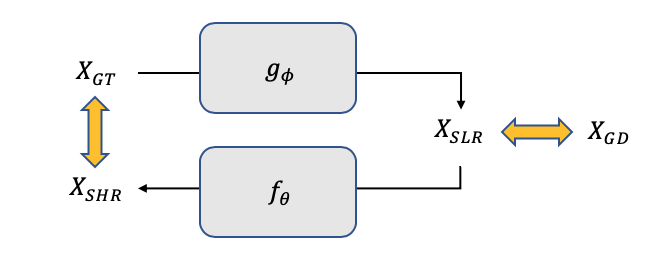
\includegraphics[width=10cm]{figures/problem}
	\caption{General \ac{TAD} problem formulation.}
  \label{fig:problem}
\end{figure}

With $g_\phi$ the downscaling and $f_\theta$ the upscaling function, $X_{GT}$ the groundtruth (input) as well as $X_{SLR}$, $X_{SHR}$ its low- and high-dimensional representation, the \ac{TAD} problem can be formulated as combined optimization problem constraining both the low-dimensional representation (readability) as well as the high-dimensional reconstruction (accuracy). While the second constraint can be easily formulated using the input image $X_{GT}$ as groundtruth the first constraint is more vague and hard to quantify. Therefore, it is assumed that the optimal latent space encoding is similar to a trivially obtained low-dimensional representation like a (bilinearly) interpolated or greyscale image. As further described in \mysecref{sec:Approach_TS} $X_{SLR}$ is thereby not derived from scratch but builds up on the guidance image in the training procedure so that both optimization problems can be solved more independently than learning both $X_{SLR}$ and $X_{SHR}$ from scratch and typically the first optimization problem (readability of $X_{SLR}$) is easier to solve for the model.

\section{Autoencoder Network Architecture}
\label{sec:Approach_ANA}
As no groundtruth for the low resolution image is available, since \ac{TAD} poses requirements for both the down- and upscaling and because it has proven to work for the \ac{TAD} problem in previous works an autoencoder design is used.

\begin{figure}[!htbp]
	\centering
	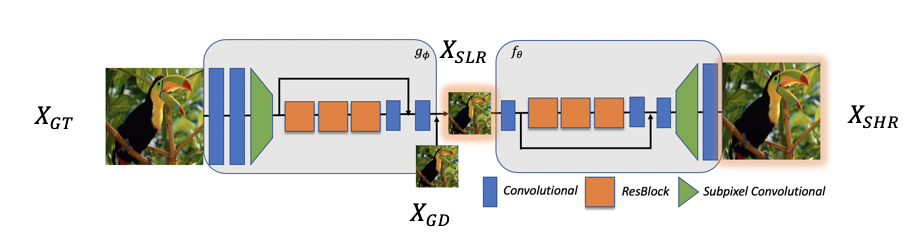
\includegraphics[width=14cm]{figures/architecture_example.png}
	\caption{Example architecture of the \ac{TAD} autoencoder network design for \ac{SISR} task.}
  \label{fig:architecture}
\end{figure}

The autoencoder should be able to handle an input image of general size, it should be runtime-efficient, store as much information as possible while downscaling as well as end-to-end and efficiently trainable.
Therefore a convolutional-only, reasonable shallow network design is used. To avoid the loss of information during downscaling instead of pooling operations subpixel convolutional layers are employed. Furthermore, in order to enable efficient training and circumvent vanishing gradient problems (especially for larger networks that were tested) next to direct forward passes ResNet (\cite{DRLFIR}) like \textit{Resblocks} are used, which are structured as

$$Resblock(x) = x + Conv2D(ReLU(Conv2D(x)))$$

Since this network design does not continuously downscale the input but
applies pixel shuffling to downscale while all other layers do not alter their inputs shape, the networks also is easily adaptable to design changes, which simplifies the architecture optimization process.

\section{Loss Function}
\label{sec:Approach_LF}
The loss function $L$ consists of two parts, representing both optimization problems introduced in \mysecref{sec:Approach_GPF}. The first one, $L_{TASK}$, is task-dependent and states the difference between the decoders output $X_{SHR}$ and the desired output $X_{GT}$, e.g. the original \ac{HR} in the \ac{SISR} task.

$$L_{TASK} = L1(X_{GT}, X_{SHR})$$

The second part, $L_{LATENT}$, encodes the human-readability of the low-dimensional representation. So $L_{LATENT}$ is the distance between the interpolated guidance image $X_{GD}$ and the actual encoding $X_{SLR}$:

$$L_{LATENT} = \begin{cases}
L1(X_{GD}, X_{SLR}) & \text{if } ||L1/d_{max}|| \geq \epsilon
\\ 0.0 & \text{otherwise}
\end{cases}$$

with $||L1/d_{max}||$ being the $L1(X_{GD}, X_{SLR})$ loss normalized
by the maximal deviation between $X_{GD}$ and $X_{SLR}$. Hence, $L_{LATENT}$ is zero in an $\epsilon$-ball around the guidance image, ensuring that \ac{SLR} is close to the guidance image but also helps to prevent overfitting to the trivial solution $X_{GD} = X_{SLR} \Leftrightarrow g_\phi = 0$. As shown in \mychapterref{sec:ExperimentsandResults} introducing an $\epsilon$-ball also improves the model's robustness against perturbations.
The overall loss function is a weighted sum of both of the loss function introduced above. The relative weight $(\alpha, \beta)$ is of large importance for the trade-off between the readability requirement and the performance of the model's upscaling part (super-resolution, colorization). However, as described above the readability requirement is less strict so that typically $\alpha >> \beta$.

$$L = \alpha L_{TASK} + \beta L_{LATENT}$$

\section{Training Specifications}
\label{sec:Approach_TS}
Even if a guidance image is part of the loss function learning both the low- and high-dimensional representation from scratch poses a combined optimization problem which usually is very hard to solve. To ensure (faster) convergence, therefore in the beginning of the training procedure the guidance image is added to the encoder's output and the encoding is not discretized (finetuning). This improves both the convergence rate of $X_{SLR}$ and $X_{SHR}$, especially in the beginning of the training procedure, since merely a difference between the interpolated representation and the more optimal encoding has the be derived and the down- and upscaling can be learned more independently since the lower dimensional representation is always guaranteed to be useful for upscaling.

\begin{figure}[!htbp]
    \centering
    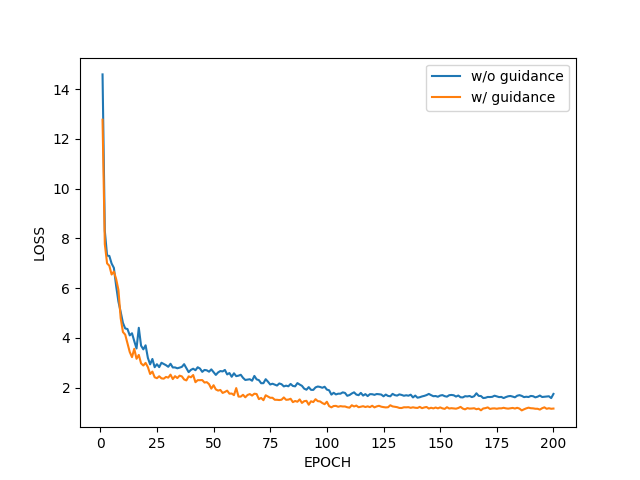
\includegraphics[height=5cm]{figures/guidance_loss.png}
    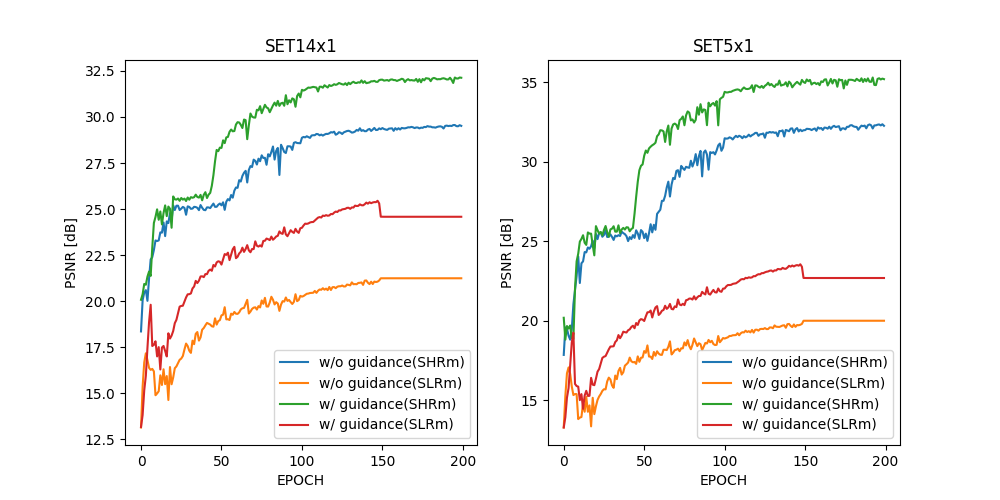
\includegraphics[height=5cm]{figures/guidance_psnrs.png}
    \caption{Loss curve without adding guidance image (left) and with
    adding guidance image (right) while training for \ac{IC} example.}
    \label{fig:loss_w_wo_adding_guidance}
\end{figure}

\begin{figure}[!htbp]
    \centering
    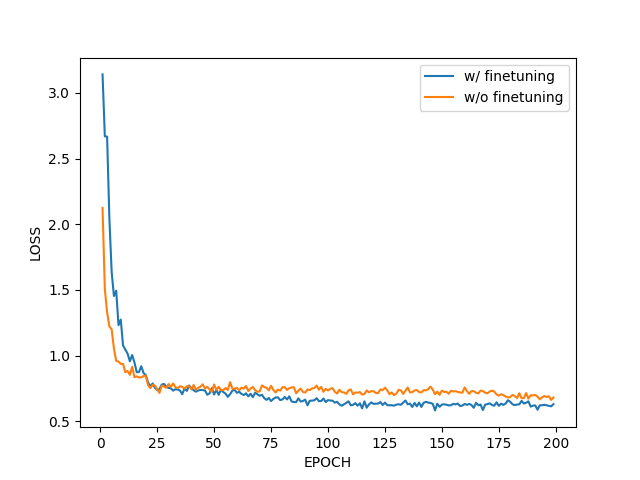
\includegraphics[height=5cm]{figures/finetuning_loss.png}
    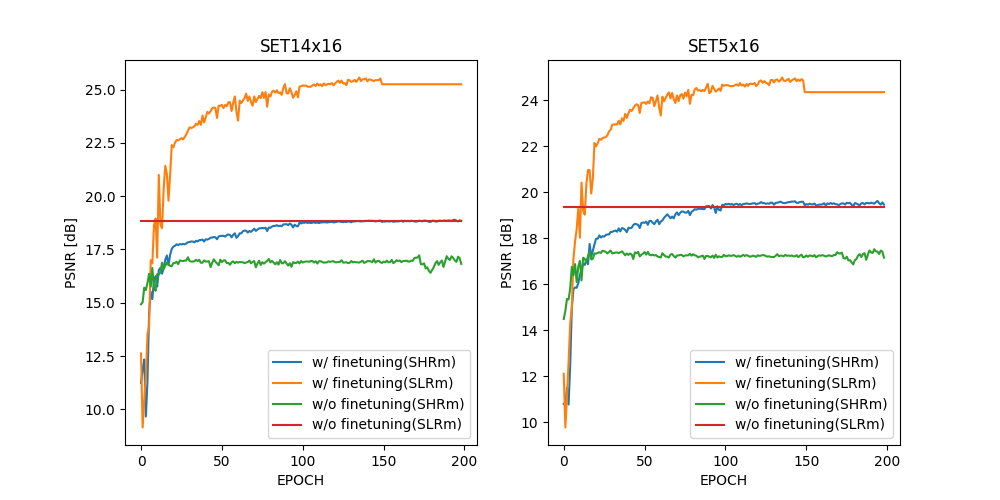
\includegraphics[height=5cm]{figures/finetuning_psnrs_16.png}
    \caption{Loss curve without finetuning (left) and with finetuning (right) while training for \ac{SISR} (scale = $16$) example.}
    \label{fig:loss_w_wo_finetuning}
\end{figure}

\section{Task-Specific Design}
\label{sec:Approach_TSD}
While the general approach derived in \mysecref{sec:Approach_GPF} can be trivially applied on the \ac{SISR} and on the \ac{IC} problem the extension to the \ac{VSR} task is more advanced. In the following the specification of all three problems are presented:

\subsection*{Single-Image-Super-Resolution Problem}
An example of the overall design of the \ac{TAD} pipeline applied on the
\ac{SISR} problem is shown in \myfigref{fig:architecture}. The high-dimensional space here is a high-resolution image ($X_{GT} = X_{HR}$), while the low-resolution guidance image is the bilinearly downscaled image ($X_{GD} = X_{LR}^{B}$). As shown for an example of scaling factor 4 in \mysecref{sec:Experiments_SISR} the model can be trained more efficiently as well as performs better when iteratively scaling (i.e. scaling two times with factor 2, instead of one time with factor 4 directly).

\subsection*{Video-Super-Resolution}
As pointed out in \mychapterref{sec:RelatedWork} the challenge of \ac{VSR} compared to \ac{SISR} is to not only take one frame into account but subsequent frames in order to reconstruct opaqued objects, reflect motions, etc. As shown in \mychapterref{sec:RelatedWork} most approaches tackling the \ac{VSR} problem follow a two-step approach, firstly reconstructing the optical flow using the current and previous low-resolution, using the result to warp the image and finally upscale it. An improvement in any of these building blocks would improve the overall reconstruction, therefore there are multiple possibilities for finding a more optimal low-dimensional representation. Several approaches were tried including a direct approach which encodes the reconstruction capability of a given \ac{VSR} model into the loss function and tries to shape the low-dimensional representation such that the model's performance improves as well as an approach directly targeting the optical flow calculation (more details in the appendix).

\begin{figure}[!htbp]
	\centering
	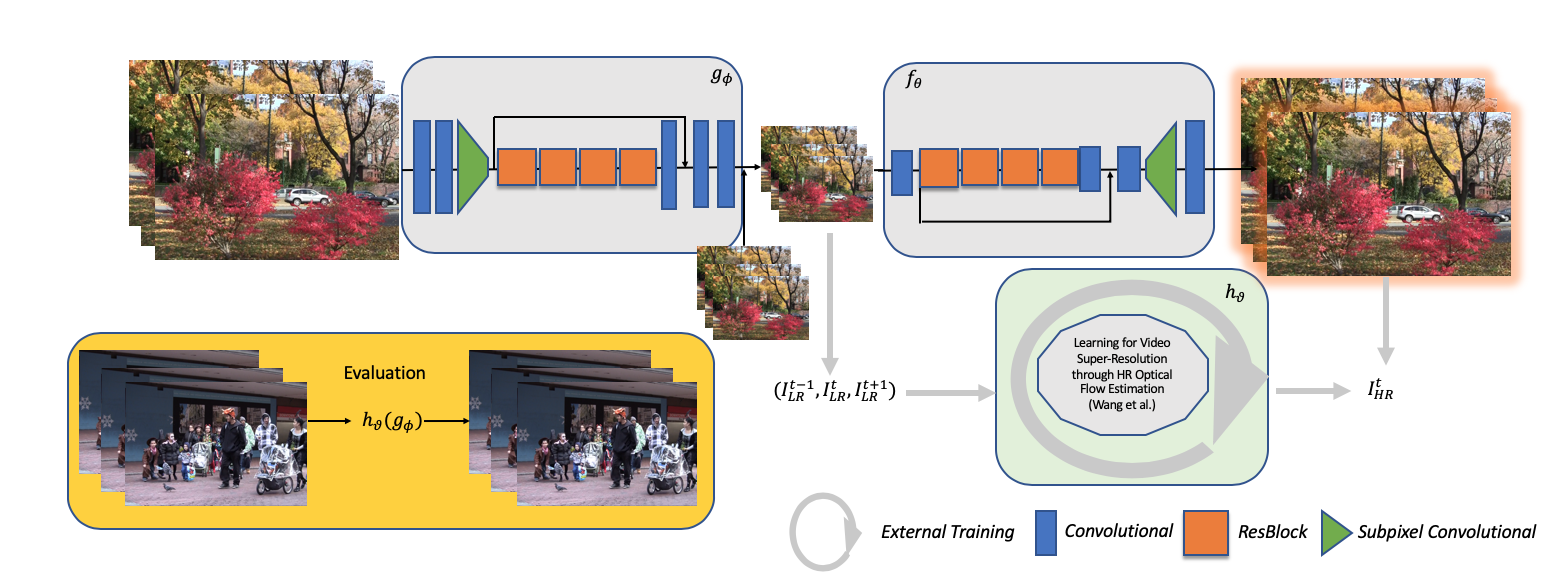
\includegraphics[width=14cm]{figures/architecture_video_external}
	\caption{Design for \ac{TAD} video super-resolution task (example network
  architecture).}
  \label{fig:architecture_video}
\end{figure}

The most promising approach is displayed in \myfigref{fig:architecture_video} and involves a training in multiple steps. In the first step, the autoencoder model is trained on incoherent images (similar to \ac{SISR}) to learn a good general down- and upscaling transformation. In a second step the pretrained model is explicitly trained on a video dataset, in order to produce the training dataset for a \ac{VSR} model, which is trained on this SLR frames specifically in the third step. After training to validate the model subsequent frames are downscaled first using the video pretrained \ac{TAD} model, the downscaled images are then fed to the trained \ac{VSR} model, upscaling them. While this approach basically is applicable to all \ac{VSR} frameworks in the scope of this project the SOFVSR (\cite{LFVSRTHROFE}) model was used. \footnote{Further details about the selection of SOFVSR and a description of the approach itself can be found in the appendix.}

\subsection*{Image Colorization}
While in a grayscale image information about intensity, color value and
saturation are mingled over all channels, other color spaces split these
information in separate channels. In order to contain as much information about the original colors a non-uniformly-weighted (while grayscale would be a uniformly weighted sum, destroying color contrast information) and static (i.e. non periodic like hue in HSV color space) sum of original color values would be optimal, which is e.g. the Y channel of the YCbCr channel. Therefore it is used as guidance image ($X_{GD} = X_{GRY}^Y$), while the original colored image can be used as groundtruth ($X_{GT} = X_{COL}$).

\begin{figure}[!htbp]
    \centering
    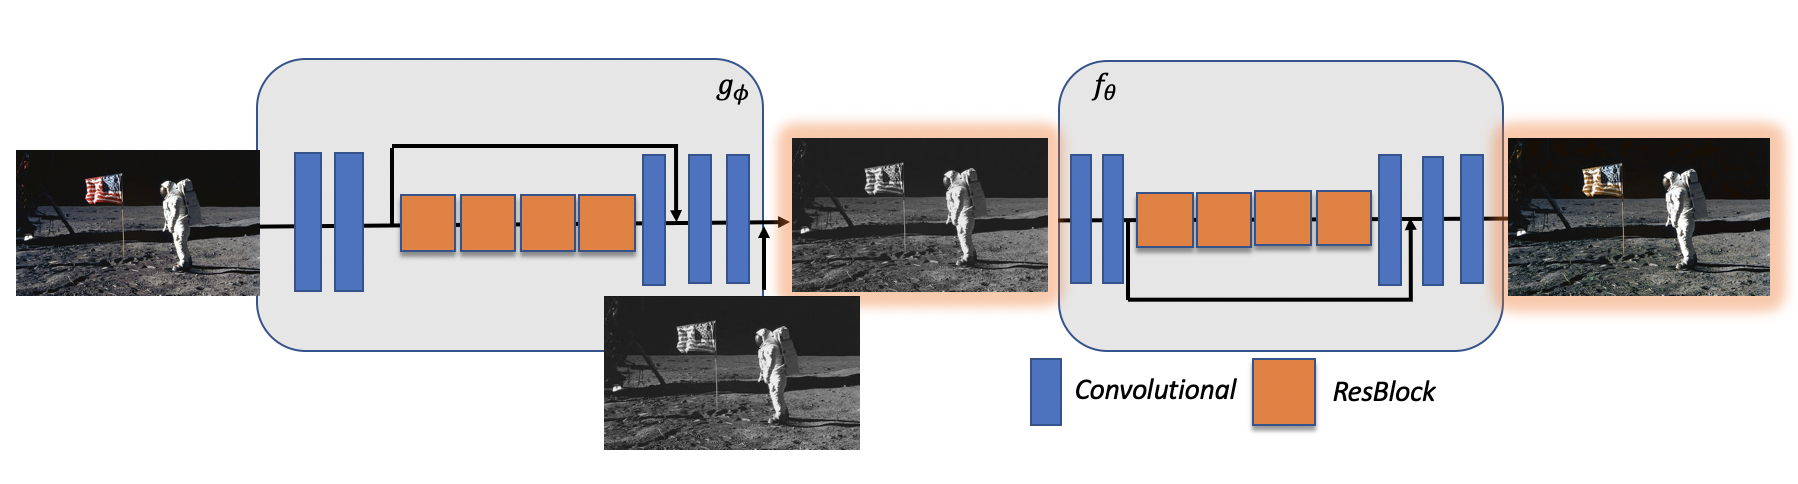
\includegraphics[width=14cm]{figures/architecture_color_large.png}
    \caption{Design for \ac{TAD} colorization task (example network architecture).}
    \label{fig:architecture_color}
\end{figure}

\section{Implementation}
\label{sec:Approach_IMP}
The project was implemented in Python 3, using the PyTorch deep learning
framework. Although some ideas from Kim et al. \cite{TAID} were adopted as described above the pipeline had to be re-implemented from scratch and
re-validated since neither code nor any pretrained model have been
available publicly (nor upon request). As PyTorch merely supports
subpixel convolutional layers, their inverse transformation was implemented as well. Since most of the open-source models for the \ac{VSR} problem merely are available in Tensorflow, as is the used model, it was re-implemented and adapted to the \ac{TAD} pipeline.
\newline
During program development it was paid attention to generality and
commutability in order to efficiently test a variety of different models and datasets as well as guarantee comparability of different approaches. The full code stack can be found on \url{https://github.com/simon-schaefer/tar}.

% The objectives of the ``Materials and Methods'' section are the following:
% \begin{itemize}
%  \item \textit{What are tools and methods you used?} Introduce the environment, in which your work has taken place - this can be a software package, a device or a system description. Make sure sufficiently detailed descriptions of the algorithms and concepts (e.g. math) you used shall be placed here.
%  \item \textit{What is your work?} Describe (perhaps in a separate section) the key component of your work, e.g. an algorithm or software framework you have developed.
% \end{itemize}
